\subsubsection{Compito C5: Salvataggio di un file della community}

Il compito C5 richiedeva all’utente di accedere alla sezione ``Community'', ricercare i documenti relativi al corso di ``CyberSecurity'', salvare uno dei file proposti all’interno della propria area personale e verificarne la corretta archiviazione. L’obiettivo era valutare l’usabilità dell’ecosistema di condivisione pubblica, con particolare attenzione all’efficacia dei filtri di ricerca, alla visibilità dei contenuti e alla chiarezza semantica dell'azione di salvataggio.

\paragraph{Analisi delle prestazioni generali}

La riprogettazione introdotta nella versione B ha generato un progresso netto e confermato sul piano statistico in tutte le metriche prestazionali del compito (Tabella~\ref{tab:6-c5-1}), ferma restando l'efficacia impeccabile registrata per tutti i partecipanti con entrambe le interfacce. L'aspetto di maggior rilievo risiede nella decisa contrazione degli errori medi commessi dagli utenti, crollati del 57,14\% (da 1,40 a 0,60) grazie a una più chiara distinzione semantica delle opzioni. A questo miglioramento si affianca un abbattimento drastico dei tempi medi di esecuzione, ridottisi del 35,48\% (da 1.26.48 a 0.56.00), e una riduzione sistematica e non attribuibile al caso del 31,84\% nel numero medio di click necessari (che scendono da 14,87 a 10,13).

Tali benefici operativi si riflettono in una diminuzione della difficoltà percepita, la cui mediana scende da 2 a 1. A supporto di questa tendenza, i punteggi medi rappresentati nella Figura~\ref{fig:6-c5-1} evidenziano una fluttuazione discendente da 2,40 a 1,80, confermando come la nuova soluzione abbia mitigato i punti di attrito cognitivo riscontrati nella prima versione.

\begin{figure}[H]
	\centering
	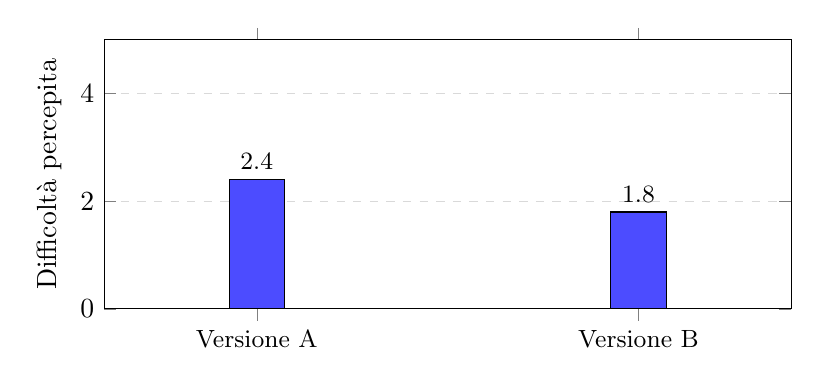
\begin{tikzpicture}
		\begin{axis}[
				ybar,
				bar width=20pt,
				width=0.85\textwidth,
				height=5cm,
				symbolic x coords={Versione A, Versione B},
				xtick=data,
				x tick label style={font=\small},
				ylabel={Difficoltà percepita},
				ymin=0, ymax=5,
				ymajorgrids=true,
				grid style={dashed, gray!30},
				enlarge x limits=0.4,
				nodes near coords,
				every node near coord/.style={font=\small, color=black},
			]
			\addplot+[
				ybar,
				fill=blue!70,
				draw=black
			] coordinates {
					(Versione A,2.40)
					(Versione B,1.80)
				};
		\end{axis}
	\end{tikzpicture}
	\caption{Confronto della difficoltà percepita tra Versione A e Versione B per C5.}
	\label{fig:6-c5-1}
\end{figure}

\begin{table}[H]
	\centering
	\footnotesize
	\renewcommand{\arraystretch}{1.2}
	\caption{Metriche prestazionali globali aggregate per il compito C5.}
	\label{tab:6-c5-1}
	\begin{tabular}{|>{\raggedright\arraybackslash}p{2.2cm}|>{\centering\arraybackslash}p{1.5cm}|>{\centering\arraybackslash}p{1.5cm}|>{\centering\arraybackslash}p{1.5cm}|>{\centering\arraybackslash}p{1.5cm}|>{\centering\arraybackslash}p{1.8cm}|>{\centering\arraybackslash}p{1.6cm}|}
		\hline
		\rowcolor{gray!30}
		\textbf{C5}           & \multicolumn{2}{c|}{\textbf{Versione A}} & \multicolumn{2}{c|}{\textbf{Versione B}} & \textbf{Variazione \%} & \textbf{Rilevanza}                                            \\ \hline
		\textit{Success Rate} & \multicolumn{2}{c|}{100,00\%}            & \multicolumn{2}{c|}{100,00\%}            & \textbf{Invariato}     &                                                               \\ \hline
		\rowcolor{gray!30}
		                      & \textbf{Media}                           & \textbf{DEV.ST}                          & \textbf{Media}         & \textbf{DEV.ST}    & \multicolumn{2}{c|}{}                    \\ \hline
		\textit{Errori}       & 1,40                                     & 1,00000                                  & 0,600                  & 1,12122            & \textbf{-57,14\%}     & \pvalue{0,01717} \\ \hline
		\textit{Tempo}        & 1.26.48                                  & 0,02323                                  & 0.56.00                & 0,02892            & \textbf{-35,48\%}     & \pvalue{0,03876} \\ \hline
		\textit{Click}        & 14,87                                    & 6,15127                                  & 10,13                  & 4,59606            & \textbf{-31,84\%}     & \pvalue{0,03767} \\ \hline
		\rowcolor{gray!30}
		                      & \multicolumn{2}{c|}{\textbf{Mediana}}    & \multicolumn{2}{c|}{\textbf{Mediana}}    & \multicolumn{2}{c|}{}                                                                  \\ \hline
		\textit{Difficoltà}   & \multicolumn{2}{c|}{2}                   & \multicolumn{2}{c|}{1}                   & \multicolumn{2}{c|}{}                                                                  \\ \hline
	\end{tabular}
\end{table}

La riduzione significativa dei tempi di completamento e degli errori indica un miglioramento sostanziale dell’efficienza complessiva del flusso di interazione. Il redesign ha ridotto le ambiguità operative e semplificato la sequenza di azioni necessarie per il salvataggio dei contenuti.

\paragraph{Analisi qualitativa: commenti e osservazioni degli utenti}

Le evidenze quantitative sono supportate dalle osservazioni raccolte durante le sessioni di test e dai protocolli \textit{thinking aloud}. Nella versione originale (A), sono emerse criticità ricorrenti:

\begin{itemize}
	\item \textbf{Ambiguità tra salvataggio e download}: gli utenti hanno frequentemente confuso l’azione di download locale con il salvataggio nella propria area personale, a causa di una distinzione semantica non sufficientemente esplicita tra i due comandi.

	\item \textbf{Scarsa visibilità dei comandi}: diversi partecipanti hanno evidenziato difficoltà nell’individuare sia l’accesso alla sezione ``Community'' sia il comando di salvataggio dei file, segnalando una bassa visibilità degli elementi interattivi principali.

	\item \textbf{Informazioni insufficienti nei risultati di ricerca}: la lista dei documenti non riportava in modo chiaro il contesto del corso di appartenenza, generando incertezza nella selezione dei file.
\end{itemize}

Per la versione post-riprogettazione (B), le osservazioni indicano un’interazione più fluida e coerente, con margini residui di miglioramento:

\begin{itemize}
	\item \textbf{Richiesta di accesso diretto al salvataggio}: alcuni utenti hanno suggerito l’introduzione di un’azione di salvataggio direttamente dalla lista dei risultati, senza necessità di aprire la preview del documento. Pur non compromettendo il task, tale passaggio è stato percepito come potenzialmente ottimizzabile.
\end{itemize}

\paragraph{Valutazione dell’effetto di apprendimento}

Analizzando i dati in base all'ordine di esecuzione (Tabella~\ref{tab:6-c5-2}), emerge un impatto significativo della familiarità con il contesto di ricerca e con la struttura della sezione.

Nel gruppo A--B, la media dei tempi di esecuzione si contrae in modo statisticamente rilevante del 58,36\% (da 1.37.40 a 0.40.40), la media degli errori si riduce del 66,67\% (da 2,00 a 0,667), e il numero medio di click diminuisce del 42,75\% (da 15,33 a 8,78). Di contro, per il gruppo B--A non si registrano variazioni sistematiche e non attribuibili al caso: i tempi medi, la media degli errori (stabile a 0,50) e la media dei click presentano fluttuazioni che non assumono rilevanza statistica. Questo comportamento suggerisce che le barriere all'usabilità poste dalla versione A rimangono elevate anche quando gli utenti hanno già familiarità con il task, limitando i benefici dell'apprendimento nel passaggio inverso.

\begin{table}[H]
	\centering
	\footnotesize
	\renewcommand{\arraystretch}{1.2}
	\caption{Confronto delle metriche prestazionali in funzione dell'ordine di esecuzione per il compito C5.}
	\label{tab:6-c5-2}
	\begin{tabular}{|>{\raggedright\arraybackslash}p{2.2cm}|>{\centering\arraybackslash}p{1.0cm}|>{\centering\arraybackslash}p{1.0cm}|>{\centering\arraybackslash}p{1.8cm}|>{\centering\arraybackslash}p{1.6cm}|>{\centering\arraybackslash}p{1.0cm}|>{\centering\arraybackslash}p{1.0cm}|>{\centering\arraybackslash}p{1.8cm}|>{\centering\arraybackslash}p{1.6cm}|}
		\hline
		\rowcolor{gray!30}
		\textbf{Metrica}              & \multicolumn{4}{c|}{\textbf{Ordine A--B}}                                                 & \multicolumn{4}{c|}{\textbf{Ordine B--A}}                                                 \\ \cline{2-9} 
		\rowcolor{gray!30}
		                              & \textbf{A}          & \textbf{B}          & \textbf{Variazione \%} & \textbf{Rilevanza}        & \textbf{B}          & \textbf{A}          & \textbf{Variazione \%} & \textbf{Rilevanza}        \\ \hline
		\textit{Tempo (Media)}        & 1.37.40             & 0.40.40             & \textbf{-58,36\%}      & \pvalue{0,00019}          & 1.19.00             & 1.10.30             & \textbf{-10,76\%}      & \pvalue{0,70331}          \\ \hline
		\textit{Errori (Media)}       & 2,00                & 0,667               & \textbf{-66,67\%}      & \pvalue{0,02220}          & 0,500               & 0,50                & \textbf{Invariato}     & \pvalue{1,00000}          \\ \hline
		\textit{Click (Media)}        & 15,33               & 8,78                & \textbf{-42,75\%}      & \pvalue{0,04728}          & 12,17               & 14,17               & \textbf{16,44\%}       & \pvalue{0,63483}          \\ \hline
		\textit{Difficoltà (Mediana)} & 2                   & 1                   &                        & \pvalue{}                 & 1,5                 & 3                   &                        & \pvalue{}                 \\ \hline
	\end{tabular}
\end{table}

La valutazione soggettiva rispecchia coerentemente questa asimmetria tra i due gruppi. Nel gruppo A--B, la mediana della difficoltà scende da 2 a 1 nel passaggio alla versione riprogettata, in linea con l'andamento delle medie raffigurate nella Figura~\ref{fig:6-c5-2} (da 2,22 a 1,78). Nel gruppo B--A, l'effetto di trascinamento negativo della versione originale è marcato: la mediana della difficoltà raddoppia passando da 1,5 a 3. Sul piano grafico, questo peggioramento si traduce nel passaggio della media da 1,83 a 2,67. Tale tendenza qualitativa conferma come l'ambiguità strutturale della versione originale continui a generare un carico cognitivo fastidioso, nonostante la competenza precedentemente acquisita con la versione B.

\begin{figure}[H]
	\centering
	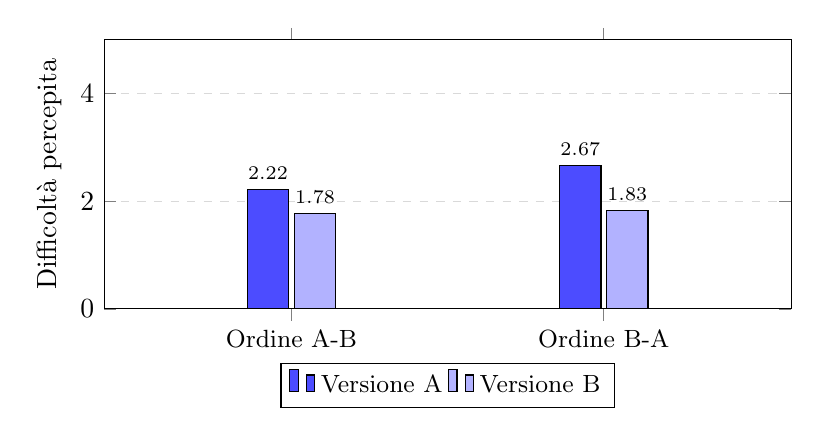
\begin{tikzpicture}
		\begin{axis}[
				ybar,
				bar width=15pt,
				width=0.85\textwidth,
				height=5cm,
				symbolic x coords={Ordine A-B, Ordine B-A},
				xtick=data,
				x tick label style={font=\small},
				ylabel={Difficoltà percepita},
				ymin=0, ymax=5,
				ymajorgrids=true,
				grid style={dashed, gray!30},
				enlarge x limits=0.6,
				legend style={at={(0.5,-0.2)}, anchor=north, legend columns=-1, font=\small},
				nodes near coords,
				every node near coord/.append style={font=\scriptsize, color=black},
			]
			\addplot+[
				fill=blue!70,
				draw=black
			] coordinates {
					(Ordine A-B,2.22)
					(Ordine B-A,2.67)
				};
			\addplot+[
				fill=blue!30,
				draw=black
			] coordinates {
					(Ordine A-B,1.78)
					(Ordine B-A,1.83)
				};
			\legend{Versione A, Versione B}
		\end{axis}
	\end{tikzpicture}
	\caption{Confronto della difficoltà percepita tra Versione A e Versione B per C5 in base all'ordine di esecuzione.}
	\label{fig:6-c5-2}
\end{figure}
